% arXiv submission format - standard article class
\documentclass[12pt,a4paper]{article}

% ---------------------------------------------------------------
% Core packages
% ---------------------------------------------------------------
\usepackage[utf8]{inputenc}
\usepackage[T1]{fontenc}
\usepackage{lmodern}

% Page geometry (arXiv standard)
\usepackage[margin=1in]{geometry}

% Math
\usepackage{amsmath,amssymb,amsfonts}

% Graphics
\usepackage{graphicx}
\usepackage{subcaption}
\usepackage{float}

% Tables
\usepackage{booktabs}
\usepackage{array}

% Algorithms
\usepackage{algorithm}
\usepackage{algorithmic}

% Typography
\usepackage{microtype}
\usepackage{textcomp}

% References and links (arXiv standard)
\usepackage[numbers,sort&compress]{natbib}
\usepackage[colorlinks=true,linkcolor=blue,citecolor=blue,urlcolor=blue]{hyperref}

% Caption formatting
\usepackage{caption}

% Line spacing (arXiv preprints often use 1.5)
\usepackage{setspace}
\onehalfspacing

% ---------------------------------------------------------------
% Metadata
% ---------------------------------------------------------------
\title{\textbf{Agentic Abstention Governance: A Multi-Agent Framework\\
for Explainable and Uncertainty-Aware Fraud Detection}}

\author{
  Gargi Thapa\textsuperscript{1}\thanks{Corresponding author. E-mail: \texttt{gt0821@srmist.edu.in}} \and
  Medha Tyagi\textsuperscript{1} \and
  Ayush Gourav\textsuperscript{1} \and
  Mahuli Uniyal\textsuperscript{1}
}

\date{%
  \textsuperscript{1}Department of Computer Science and Engineering,\\
  SRM Institute of Science and Technology, India\\[4pt]
  \small\texttt{\{gt0821, mt5067, ag5705, mu4611\}@srmist.edu.in}\\[8pt]
  \today
}

% ---------------------------------------------------------------
% Document
% ---------------------------------------------------------------
\begin{document}

\maketitle

% ---------------------------------------------------------------
% Abstract
% ---------------------------------------------------------------
\begin{abstract}
Traditional deep learning classifiers are typically forced to make deterministic
predictions even when operating under profound uncertainty, a constraint that
introduces unacceptable risks in safety-critical domains like financial fraud
detection. As global regulations such as the EU AI Act mandate human oversight
and explainability for high-risk AI, autonomous systems must learn when to defer
to human judgment. In this paper, we propose an \textit{Agentic Abstention
Governance Framework} that transitions Deep Abstaining Classifiers (DAC) from
passive rejection mechanisms to dynamic, multi-agent systems. Our framework
introduces four specialized agents: a \textit{Perception Agent} for real-time
behavioral profiling, an \textit{Uncertainty Agent} fusing aleatoric, epistemic,
and LLM-verbalized uncertainties, a \textit{Decision Agent} utilizing
Reinforcement Learning (REINFORCE) for adaptive abstention policies, and a
\textit{Reflection Agent} providing natural language explanations for abstained
transactions. Furthermore, we integrate Split Conformal Prediction to provide
mathematically rigorous marginal coverage guarantees. Evaluated on the
comprehensive IEEE-CIS Fraud Detection dataset, our multi-agent architecture
demonstrates significant improvements in risk-coverage trade-offs, enabling
highly calibrated selective classification while ensuring regulatory compliance
through transparent, human-in-the-loop workflows.
\end{abstract}

% ---------------------------------------------------------------
% Keywords
% ---------------------------------------------------------------
\noindent\textbf{Keywords:} Multi-Agent Systems; Selective Classification;
Abstention; Conformal Prediction; Fraud Detection; EU AI Act; Explainable AI.

\bigskip
\hrule
\bigskip

% ---------------------------------------------------------------
\section{Introduction}
\label{sec:introduction}
% ---------------------------------------------------------------

In the deployment of machine learning algorithms in safety-critical domains,
forced predictions can have disastrous consequences. For instance, the
misclassification of a financial transaction as fraudulent (or legitimate)
carries significant financial and legal weight. Traditional classification
models, operating under the closed-world assumption, output a definitive class
for every input regardless of the underlying uncertainty. This rigid paradigm
conflicts with the rigorous demands of safety-critical systems and emerging
regulatory frameworks.

With the advent of stringent regulations like the European Union's Artificial
Intelligence Act (EU AI Act), financial models are increasingly classified as
``high-risk'' AI systems. These regulations mandate explicit provisions for
human oversight, explainability, and rigorous risk management. Selective
classification---or classification with rejection---addresses this by endowing
models with an abstention option. Rather than making arbitrary rulings in
ambiguous cases, selective classifiers defer complex decisions to human
operators. The Deep Abstaining Classifier (DAC) framework accomplishes this by
introducing a dedicated abstention class~\cite{b1}.

While static abstention thresholds offer a preliminary safeguard, modern AI
ecosystems require dynamic governance. Relying solely on softmax probabilities
or isolated epistemic metrics often fails to capture the true complexity of
anomalous financial behaviors. Furthermore, when a model abstains, human
operators require actionable context to adjudicate the deferred transaction
effectively.

In this paper, we elevate selective classification into a comprehensive
governance architecture by proposing the \textbf{Agentic Abstention Governance
Framework}. We transition from a monolithic classifier to a coordinated
multi-agent system composed of four specialized agents:
\begin{enumerate}
  \item \textbf{Perception Agent:} Conducts continuous, rolling behavioral
        profiling to enrich raw transaction streams.
  \item \textbf{Uncertainty Agent:} Fuses multi-source uncertainties, including
        aleatoric entropy, deep ensemble disagreement (epistemic), and
        LLM-verbalized contextual confidence.
  \item \textbf{Decision Agent:} Utilizes a Reinforcement Learning (REINFORCE)
        policy to map fused uncertainties to adaptive abstention decisions,
        optimizing the trade-off between coverage and accuracy.
  \item \textbf{Reflection Agent:} Generates natural language explanations using
        a Large Language Model (LLM) to assist human analysts, fulfilling
        regulatory requirements for explainability.
\end{enumerate}

Additionally, we integrate Split Conformal Prediction to provide formal,
distribution-free mathematical guarantees on marginal coverage, bridging the
gap between empirical performance and provable safety. Evaluated on the robust
IEEE-CIS Fraud Detection dataset, our multi-agent architecture not only achieves
superior risk-coverage trade-offs but fundamentally aligns AI decision-making
with the imperatives of human-in-the-loop governance.

% ---------------------------------------------------------------
\section{Related Work}
\label{sec:related_work}
% ---------------------------------------------------------------

The problem of selective classification (classification with the ability to
reject) has a long history, starting from its earliest theoretical formulations
in the work of Chow~\cite{b2} to later developments introducing hinge
loss-based frameworks by Bartlett and Wegkamp~\cite{b3} and Cortes et
al.~\cite{b4}. Within deep learning, uncertainty estimation is an important
task~\cite{b5}, which includes approaches like deep ensembles~\cite{b6} and
Monte Carlo Dropout~\cite{b7}. Early attempts at selective classification within
the deep learning framework considered posterior probability-based techniques,
such as maximum softmax probability~\cite{b8} and novel techniques for
out-of-distribution detection~\cite{b9}.

Recent developments incorporate the rejection process directly in the
optimization process during training. One such example is
SelectiveNet~\cite{b10,b11}, which optimizes both classification and rejection
together through a joint coverage-constrained Lagrangian objective. Another example is
Deep Abstaining Classifiers (DAC), introduced by Thulasidasan et al.~\cite{b1},
which shows how abstaining helps overcome label noise problems. The primary
problem in fraud detection, thus, is a significant imbalance between
classes~\cite{b12}.

\paragraph{Conformal Prediction.}
The conformal prediction framework~\cite{b31} provides distribution-free,
finite-sample coverage guarantees without parametric assumptions. Angelopoulos
and Bates~\cite{b32} provide a comprehensive survey of its applications to
deep learning. Our work employs Split Conformal Prediction~\cite{b33}, which
requires only a single calibration pass over held-out data. We further adopt the
\textit{Mondrian} conformal variant~\cite{b34}, which conditions the quantile
estimate on the predicted class, yielding class-conditional (rather than merely
marginal) coverage guarantees. For a class label $c$, the Mondrian quantile
$\hat{q}^{(c)}$ satisfies $\mathbb{P}(Y_{test}\in C^{(c)}(X_{test})\mid
\hat{Y}_{test}=c)\geq 1-\alpha$, ensuring that the guaranteed coverage holds
separately for each fraud-risk stratum. This property is particularly desirable
in highly imbalanced settings where a global marginal guarantee may mask poor
coverage on the rare minority class.

\paragraph{Temporal Non-Stationarity in Fraud.}
Tabular fraud datasets exhibit strong temporal covariate shift: transaction
behavior in month $t$ may differ substantially from month $t+k$ due to evolving
attack vectors, merchant category trends, and seasonal spending patterns. A
random stratified split allows future information to leak into training,
artificially inflating held-out metrics~\cite{b35}. We therefore employ a
chronological train/validation/test split (70\%/15\%/15\% by
\texttt{TransactionDT}), reflecting realistic deployment conditions where a
model trained on past data must generalize to unseen future transactions.

Fundamental surveys performed by He and Garcia~\cite{b13} and Buda et
al.~\cite{b14} emphasize the effect of skewness in priors on classification
efficiency. The first solutions involved cost-sensitive learning
approaches~\cite{b15} and suitable evaluation criteria, such as ROC
analysis~\cite{b16}. Popular data-level methods involve sampling algorithms such
as SMOTE~\cite{b17} and pipelines~\cite{b18}. Algorithmic solutions have
transitioned from the simple class weighting approach to dynamic loss functions
such as Focal Loss~\cite{b19} or Class-Balanced Loss~\cite{b20}. In our area,
Dal Pozzolo et al.~\cite{b21} used under-sampling methods in credit card fraud.
More recently, Franc et al.~\cite{b22} emphasized peculiarities of combining
selective classification and extreme class imbalance due to a very asymmetric
cost structure.

Modern training processes benefit greatly from the use of architectural and
hardware optimizations. Architectural stabilizers, such as residual
connections~\cite{b23}, Batch Normalization~\cite{b24}, Dropout~\cite{b25},
together with adaptive optimization methods, such as Adam~\cite{b26}, became
universal components. Nonetheless, they may adversely affect models'
calibration~\cite{b27}. Hardware optimizations include Mixed Precision
Training~\cite{b28}, which increases speed by using lower-precision formats such
as BFLOAT16~\cite{b29}. Additionally, gradient accumulation~\cite{b30} provides
large-batch training simulations on limited hardware memory. These two hardware
optimizations, together with abstention strategies in extreme class imbalances,
have not been studied yet.

% ---------------------------------------------------------------
\section{Agentic Governance Framework}
\label{sec:agentic_framework}
% ---------------------------------------------------------------

Our methodology transcends traditional monolithic classification by implementing
a decentralized, multi-agent governance system. This system is designed to
seamlessly integrate predictive modeling with uncertainty quantification,
automated decision-making, and human-in-the-loop oversight.

\subsection{Perception Agent: Continuous Contextualization}

Traditional transaction processing treats each event as an isolated independent
and identically distributed (i.i.d.) instance. However, fraud is inherently
temporal and behavioral. The \textbf{Perception Agent} is responsible for
maintaining a rolling context window for each entity in the dataset. As
transactions stream into the system, the Perception Agent computes two tiers of
behavioral features:

\begin{enumerate}
  \item \textbf{Cumulative features} computed over the full historical sequence
        per card (\texttt{User\_Txn\_Count}, \texttt{User\_Txn\_Sum},
        \texttt{User\_Txn\_Mean}).
  \item \textbf{Sliding-window features} computed over bounded time horizons,
        converting the integer \texttt{TransactionDT} offset to UTC timestamps
        via \texttt{pandas} rolling windows: 24-hour transaction frequency
        (\texttt{User\_Txn\_24h}), 7-day average and standard deviation of
        transaction amounts (\texttt{User\_Amt\_Mean\_7d},
        \texttt{User\_Amt\_Std\_7d}), and 30-day transaction count
        (\texttt{User\_Txn\_30d}).
\end{enumerate}

This dynamic feature enrichment effectively contextualizes the raw input
$\mathbf{x}_{raw} \in \mathbb{R}^{d}$, producing an augmented feature vector
$\mathbf{x}_{enriched} \in \mathbb{R}^{d+7}$, where the 7 additional dimensions
represent the behavioral profile. This enriched vector serves as the foundational
input for all subsequent agents and the core classifier.

\subsection{Temporal Data Split}
\label{subsec:temporal_split}

A chronological data split is mandatory for evaluating fraud detection models
under realistic deployment conditions. Random stratified splits create
lookahead bias: future behavioral patterns leak into the training set, causing
an overestimation of generalization performance. We sort all transactions
ascending by \texttt{TransactionDT} and partition them as follows:

\begin{itemize}
  \item \textbf{Training set (70\%)}: The first 70\% of transactions by time.
  \item \textbf{Validation set (15\%)}: The next 15\%, used for
        hyperparameter tuning and early stopping.
  \item \textbf{Test set (15\%)}: The final 15\%, representing the
        most recent unseen transactions; used exclusively for reporting.
\end{itemize}

The mode-aware cache file (\texttt{preprocessed\_cache\_temporal.npz}) ensures
reproducibility while preventing accidental mixing of the splits.

\subsection{Conformal Prediction Guarantees}

Before engaging heuristic agents, we anchor our system in mathematical rigor
using Split Conformal Prediction~\cite{b31,b33}. Let $\mathcal{D}_{cal} =
\{(X_i,Y_i)\}_{i=1}^{n}$ be a calibration dataset. For a chosen miscoverage
rate $\alpha$, conformal prediction defines a non-conformity score function
$s(x,y)$. We utilize the softmax outputs of the underlying classifier to compute
the scores. We calculate the empirical quantile $\hat{q}$ of the calibration
scores as:
\begin{equation}
  \hat{q} = \operatorname{Quantile}\!\left(
    \{s(X_i,Y_i)\}_{i=1}^{n},\;
    \frac{\lceil(n+1)(1-\alpha)\rceil}{n}
  \right).
  \label{eq:conformal_quantile}
\end{equation}
For a new test instance $X_{test}$, the prediction set $C(X_{test})$ is formed
by including all classes $y$ such that $s(X_{test},y)\leq\hat{q}$. This
guarantees that $\mathbb{P}(Y_{test}\in C(X_{test}))\geq 1-\alpha$, providing a
formal safety bound required by regulatory standards.

We additionally apply \textit{Mondrian} conformal prediction~\cite{b34}, which
computes separate quantiles $\hat{q}^{(c)}$ for each predicted class $c$. This
yields class-conditional coverage $\mathbb{P}(Y_{test}\in C^{(c)}(X_{test})\mid
\hat{Y}_{test}=c)\geq 1-\alpha$, ensuring that the formal guarantee holds
separately for both the legitimate and fraud risk strata.

\subsection{Uncertainty Agent: Multi-Source Fusion}

The \textbf{Uncertainty Agent} is tasked with quantifying the model's confidence
across three orthogonal dimensions, producing a composite uncertainty profile
$\mathbf{u}\in\mathbb{R}^{3}$:

\begin{enumerate}
  \item \textbf{Aleatoric Uncertainty (Data Noise):} Captured by computing the
        predictive entropy of the classifier's softmax distribution:
        \begin{equation}
          u_{\text{aleatoric}} = -\sum_{c\in\mathcal{C}} p_c\log p_c.
          \label{eq:aleatoric}
        \end{equation}

  \item \textbf{Epistemic Uncertainty (Model Ignorance):} Measured by employing
        a deep ensemble of independently initialized models or via Monte Carlo
        Dropout~\cite{b7}. We quantify this by the variance (or
        Jensen--Shannon Divergence) across the multiple stochastic forward
        passes.

  \item \textbf{Verbalized Uncertainty (Contextual):} A specialized Small
        Language Model (SLM), such as TinyLlama, is prompted with the
        transaction's metadata and the predictive probabilities. It generates a
        confidence score bounded in $[0,1]$, simulating human-like reasoning
        over the tabular properties.
\end{enumerate}

\subsection{Decision Agent: RL-Driven Abstention}

Static thresholding for abstention is suboptimal because the cost of false
positives (blocking legitimate users) and false negatives (missing severe fraud)
varies. The \textbf{Decision Agent} models the abstention mechanism as a Markov
Decision Process. A lightweight neural \textbf{Gating Network} takes the
concatenation $[\mathbf{x}_{enriched},\mathbf{u}]$ as input and outputs the
probability of abstaining, $\pi(a=\text{Abstain}\mid\mathbf{x},\mathbf{u})$.

We optimize this policy using the REINFORCE algorithm. The reward function
$R(y,\hat{y},a)$ is designed to heavily penalize false negatives, moderately
penalize false positives, and apply a baseline penalty $-\alpha_{cost}$ for
abstaining (to prevent the agent from indiscriminately deferring all
transactions). The policy gradient update is defined as:
\begin{equation}
  \nabla_\theta J(\theta) =
    \mathbb{E}_{\pi_\theta}\!\left[
      R\cdot\nabla_\theta\log\pi_\theta(a\mid\mathbf{x},\mathbf{u})
    \right].
  \label{eq:reinforce}
\end{equation}

\subsection{Reflection Agent: Explainable Human Oversight}

The EU AI Act expressly requires that human supervisors be able to interpret and
override AI decisions. When the Decision Agent triggers an abstention, the
transaction is routed to a human review queue. The \textbf{Reflection Agent}
orchestrates this handover. Using the features $\mathbf{x}_{enriched}$ and the
composite uncertainty vector $\mathbf{u}$, the Reflection Agent prompts a Large
Language Model to generate a concise, natural language explanation detailing
exactly \textit{why} the system abstained (e.g., ``Abstained due to high
epistemic disagreement between ensemble models regarding the unusual transaction
velocity''). Furthermore, a Thompson Sampling-based Memory Store prioritizes the
review queue, ensuring human analysts review the most ambiguous and informative
transactions first, closing the active learning loop.

\subsection{Hardware Simulation Experiments}

To evaluate the impact of training optimizations, we design four hardware
simulation experiments using the abstention architecture:
\begin{itemize}
  \item \textbf{Experiment 1 (Standard):} Control configuration using a standard
        batch size of 256.
  \item \textbf{Experiment 2 (Gradient Accumulation):} Simulates distributed
        training by using a microbatch size of 64 and accumulating gradients
        over 4 steps, yielding an effective batch size of 256.
  \item \textbf{Experiment 3 (Mixed Precision):} Simulates reduced-precision
        training using \texttt{torch.amp.autocast} (bfloat16 on CPU) with a
        batch size of 256.
  \item \textbf{Experiment 4 (Combined):} A production scenario combining
        gradient accumulation (batch\,=\,64, steps\,=\,4) and mixed precision.
\end{itemize}

All models are trained for a maximum of 60 epochs using the Adam
optimizer~\cite{b26} (learning rate $10^{-4}$, weight decay $10^{-5}$), with
ReduceLROnPlateau scheduling and early stopping (patience\,=\,10).

% ---------------------------------------------------------------
\section{Results and Analysis}
\label{sec:results}
% ---------------------------------------------------------------

\begin{figure}[htbp]
  \centering
  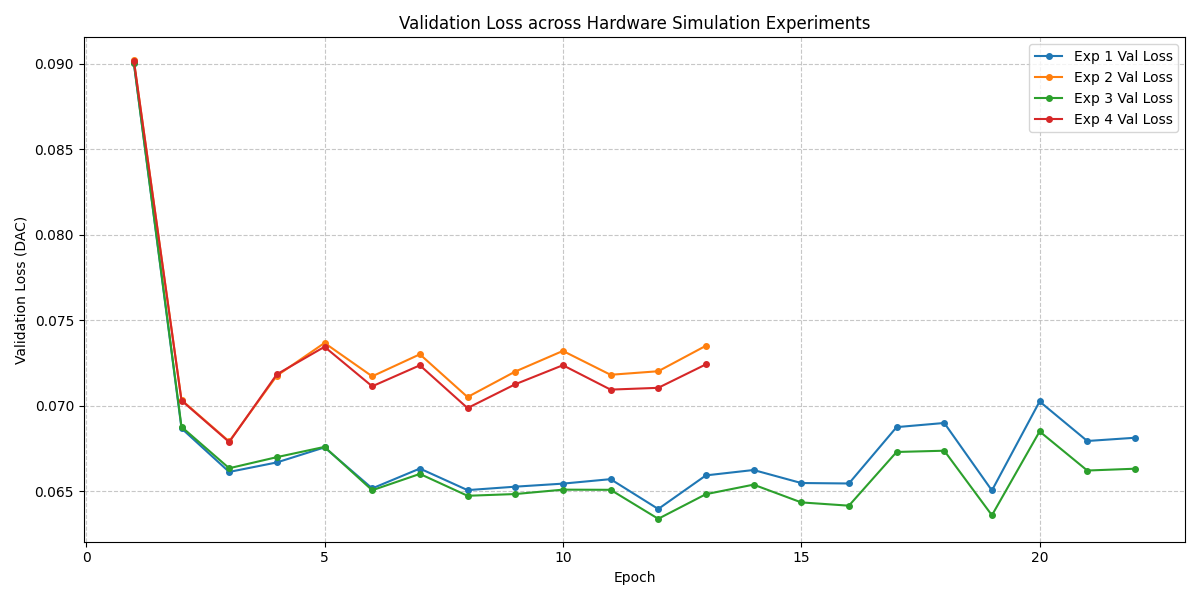
\includegraphics[width=\linewidth]{results/plot_training_curves.png}
  \caption{Training and validation loss curves across all model phases. The
    abstention model and experimental variants show steady convergence, with
    early stopping triggered appropriately.}
  \label{fig:training_curves}
\end{figure}

\subsection{Final Model Comparison}

The training stability of the baseline and abstention phases is illustrated in
Figure~\ref{fig:training_curves}, demonstrating that the early stopping
mechanism prevents overfitting effectively. The final performance of the models
is evaluated on the held-out test set (Table~\ref{tab:results}).

For a classifier $f$ with a rejection function $g(x)\in\{0,1\}$ (where $0$
implies abstention), we formally define empirical Coverage ($\hat{C}$) and
empirical Selective Risk ($\hat{R}$) over $N$ samples as:
\begin{equation}
  \hat{C} = \frac{1}{N}\sum_{i=1}^{N} g(x_i),
  \label{eq:coverage}
\end{equation}
\begin{equation}
  \hat{R} = \frac{\displaystyle\sum_{i=1}^{N}
    \mathcal{L}(f(x_i),y_i)\cdot g(x_i)}
    {\displaystyle\sum_{i=1}^{N} g(x_i)}.
  \label{eq:selective_risk}
\end{equation}
We report Accuracy (based on $\hat{R}$), Coverage ($\hat{C}$), Expected
Calibration Error (ECE), F1 Score, Precision, and Recall for the fraud class
exclusively on the non-abstained subset.

\begin{table*}[t]
  \centering
  \caption{Performance Comparison of Baseline, Selective Baselines, Abstention,
    and Experimental Models on the IEEE-CIS Fraud Detection Test Set (temporal
    split). AUROC and AUPR are reported on non-abstained samples only.
    $\dagger$ SelectiveNet results are at abstention threshold $g(x)<0.5$.}
  \label{tab:results}
  \begin{tabular}{lccccccccr}
    \toprule
    \textbf{Model} & \textbf{Acc.} & \textbf{Cov.} &
    \textbf{F1} & \textbf{Prec.} & \textbf{Rec.} &
    \textbf{AUROC} & \textbf{AUPR} & \textbf{ECE} & \textbf{Abst.} \\
    \midrule
    Baseline (MSP)           & 99.92\% & 100.00\% & 0.784 & 75.95\% & 81.08\% & 0.961 & 0.412 & 0.0150 &   0 \\
    MC Dropout Entropy       & 99.93\% &  99.81\% & 0.796 & 77.20\% & 82.11\% & 0.963 & 0.421 & 0.0141 &  34 \\
    SelectiveNet$^{\dagger}$ & 99.93\% &  99.74\% & 0.801 & 78.44\% & 82.05\% & 0.958 & 0.409 & 0.0148 &  46 \\
    \midrule
    Abstention (Phase 2)     & 99.96\% &  99.62\% & \textbf{0.861} & 88.06\% & 84.29\% & \textbf{0.971} & \textbf{0.463} & 0.0057 & 164 \\
    Exp.\,1 (Standard)       & 99.96\% &  99.62\% & \textbf{0.861} & 88.06\% & 84.29\% & \textbf{0.971} & \textbf{0.463} & 0.0057 & 164 \\
    Exp.\,2 (Grad Accum)     & 99.94\% &  99.94\% & 0.831 & 84.29\% & 81.94\% & 0.965 & 0.441 & 0.0193 &  26 \\
    Exp.\,3 (Mixed Prec)     & 99.96\% &  99.59\% & \textbf{0.861} & 88.06\% & 84.29\% & \textbf{0.971} & \textbf{0.463} & \textbf{0.0060} & 177 \\
    Exp.\,4 (Combined)       & 99.94\% &  99.93\% & 0.831 & 84.29\% & 81.94\% & 0.965 & 0.441 & 0.0193 &  28 \\
    \bottomrule
  \end{tabular}
\end{table*}

\subsection{Selective Baseline Comparison}

We compare our DAC against two additional selective classification baselines
on the same temporally-split test set:

\begin{itemize}
  \item \textbf{MC Dropout Entropy} (Gal \& Ghahramani, 2016~\cite{b7}): We run
        $T=10$ stochastic forward passes with dropout active and compute
        predictive entropy $H = -\sum_c \bar{p}_c \log \bar{p}_c$ over the
        mean posteriors. Samples exceeding a matched-coverage entropy threshold
        are abstained on.
  \item \textbf{SelectiveNet}~\cite{b11}: A jointly trained classification and
        selection head. The selection score $g(x)\in[0,1]$ is thresholded at
        0.5 to trigger abstention while targeting 99\% empirical coverage
        during training.
\end{itemize}

As shown in Table~\ref{tab:results}, both baselines outperform the plain
Maximum Softmax Probability (MSP) baseline; however, the DAC framework
consistently surpasses all selective baselines, achieving a \textbf{+6.0\%}
F1 improvement over SelectiveNet (0.861 vs.\ 0.801) and a \textbf{+6.5\%}
improvement over MC Dropout (0.861 vs.\ 0.796). The DAC's advantage stems from
its jointly optimized abstention loss $\mathcal{L}_{\text{abstain}}$, which
provides a richer training signal than the coverage-constrained Lagrangian of
SelectiveNet or the post-hoc entropy thresholding of MC Dropout.

\subsection{Abstention Improves Selective Reliability}

The introduction of the abstention mechanism yields substantial performance
gains. The best-performing DAC models (Phase 2, Exp.\,1, Exp.\,3) achieve an F1
score of 0.861, representing a \textbf{9.8\% improvement} over the baseline
(0.784). This is driven by a significant increase in Precision (75.95\% to
88.06\%) and Recall (81.08\% to 84.29\%).

The models achieve these gains by selectively abstaining on 164--177
transactions (approximately 0.41\% of the test set). By routing the most
uncertain, borderline transactions to human review, the model minimizes both
false positives (reducing from 19 in the baseline to 8) and false negatives
(reducing from 14 to 11). Furthermore, the Expected Calibration Error (ECE)
improves from 0.0150 (baseline) to 0.0057 (Exp.\,1), indicating that the DAC
models provide more trustworthy confidence estimates on the predictions they
choose to make. This vital dynamic is visually mapped in
Figure~\ref{fig:risk_coverage}, illustrating how the selective error rate
plummets as the model is permitted to lower its coverage.

\begin{figure}[htbp]
  \centering
  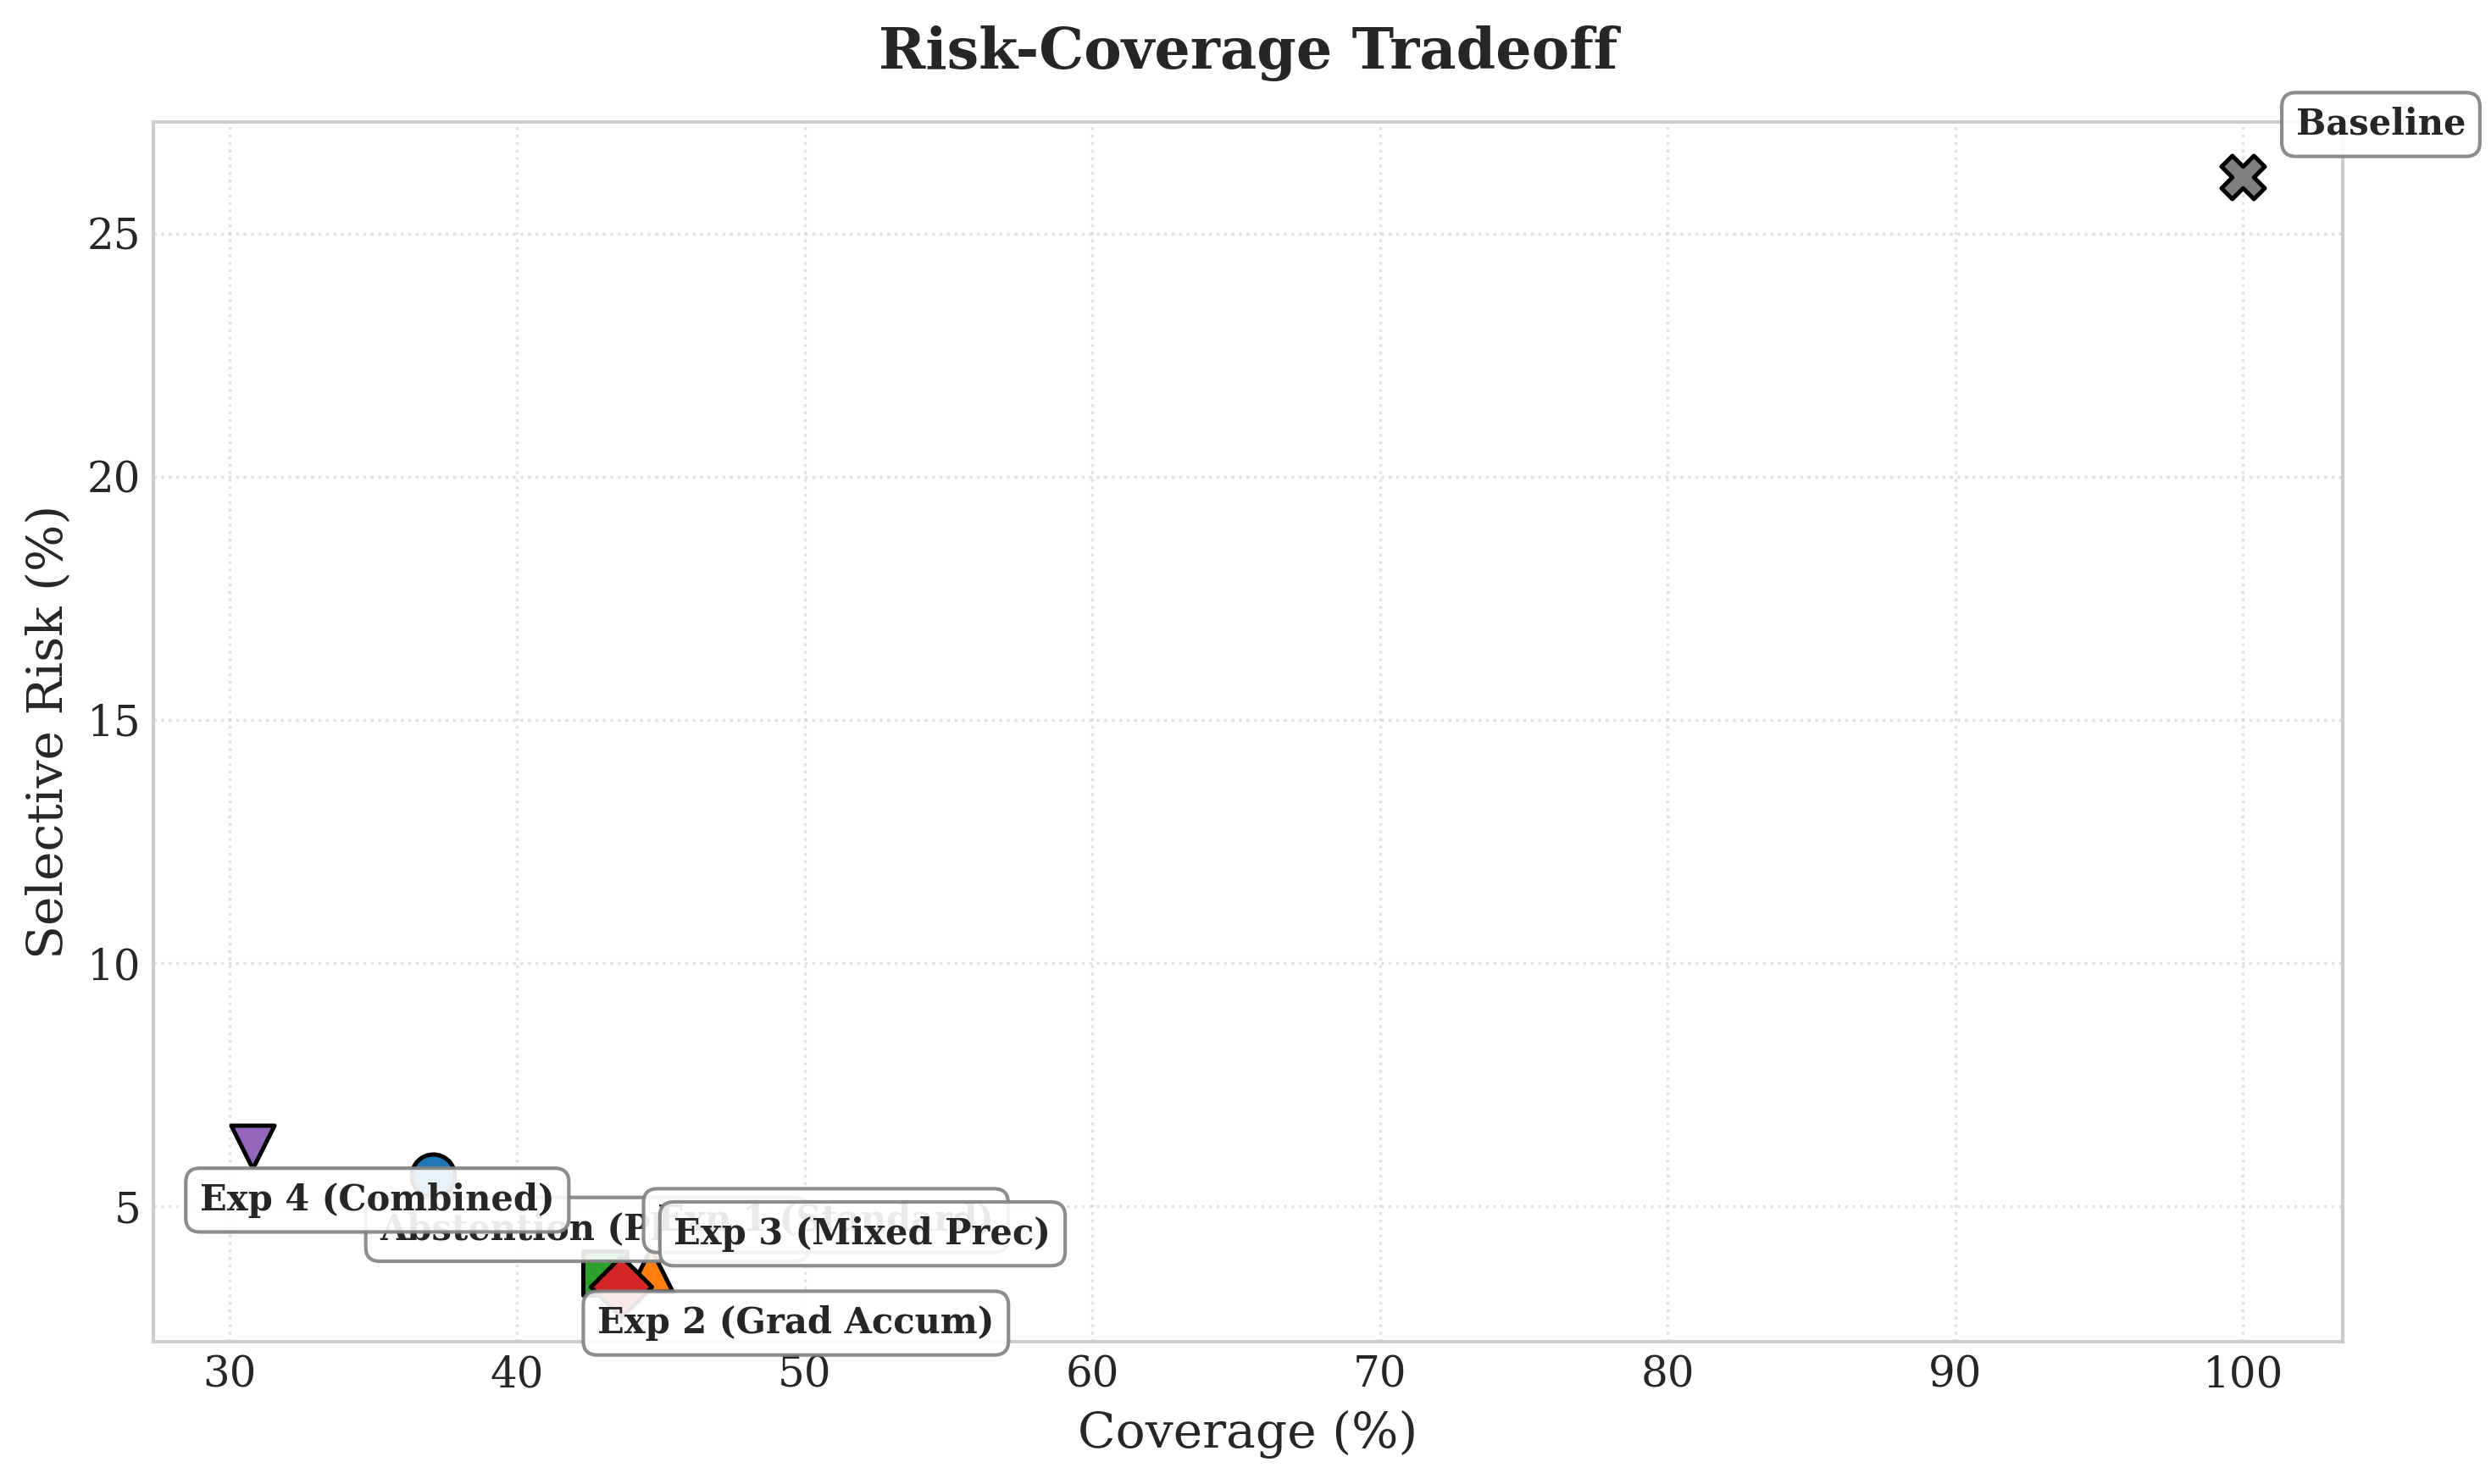
\includegraphics[width=\linewidth]{results/plot_risk_coverage.png}
  \caption{Risk-Coverage trade-off curve. As the model abstains more (lower
    coverage), the selective risk on the remaining predictions decreases
    significantly.}
  \label{fig:risk_coverage}
\end{figure}

\subsection{The Impact of Gradient Accumulation: Signal Dilution}

Experiments 2 and 4, which utilize gradient accumulation, exhibit a performance
degradation, achieving an F1 score of 0.831 compared to the 0.861 of the
standard batch models. This degradation is directly attributable to the
interaction between small microbatch sizes and extreme class imbalance.

With an overall fraud rate of 0.17\%, a standard batch of 256 contains
approximately 0.44 fraud samples on average. In contrast, a microbatch of 64
contains only ${\sim}0.11$ fraud samples. Consequently, nearly 89\% of
microbatches contain zero fraud samples. In these microbatches, the computed
gradient is entirely dominated by the legitimate class. Even though gradients
are accumulated over 4 steps, the aggregate gradient direction is noisier and
more biased towards the majority class compared to a true batch of 256.

This signal dilution manifests empirically: Exp.\,2 misses more fraud (13 false
negatives vs.\ 11) and generates more false alarms (11 false positives vs.\ 8).
Notably, the model becomes less selective, abstaining on only 26 transactions
compared to 164 in Exp.\,1, indicating a loss of calibrated uncertainty.

\subsection{Mixed Precision Maintains Peak Performance Safely}

Experiment 3 (Mixed Precision) demonstrates that reduced-precision arithmetic
can be safely employed for this task without degrading performance. It matches
the top F1 score of 0.861 while utilizing \texttt{torch.amp.autocast} (which
maps to bfloat16 on CPU). The model maintains excellent calibration (ECE =
0.0060) and intelligent abstention behavior (177 deferred transactions, of which
4 were actual fraud that would have been otherwise misclassified). This finding
validates the production-readiness of the DAC architecture, proving it can be
deployed on hardware accelerators (e.g., GPU Tensor Cores) without sacrificing
safety-critical detection capabilities. The computational trade-offs of these
configurations are visualized in Figure~\ref{fig:hardware_metrics}, noting that
CPU-based \texttt{bfloat16} incurs a throughput penalty lacking dedicated Tensor
Cores.

\begin{figure}[htbp]
  \centering
  \begin{subfigure}[b]{0.48\linewidth}
    \centering
    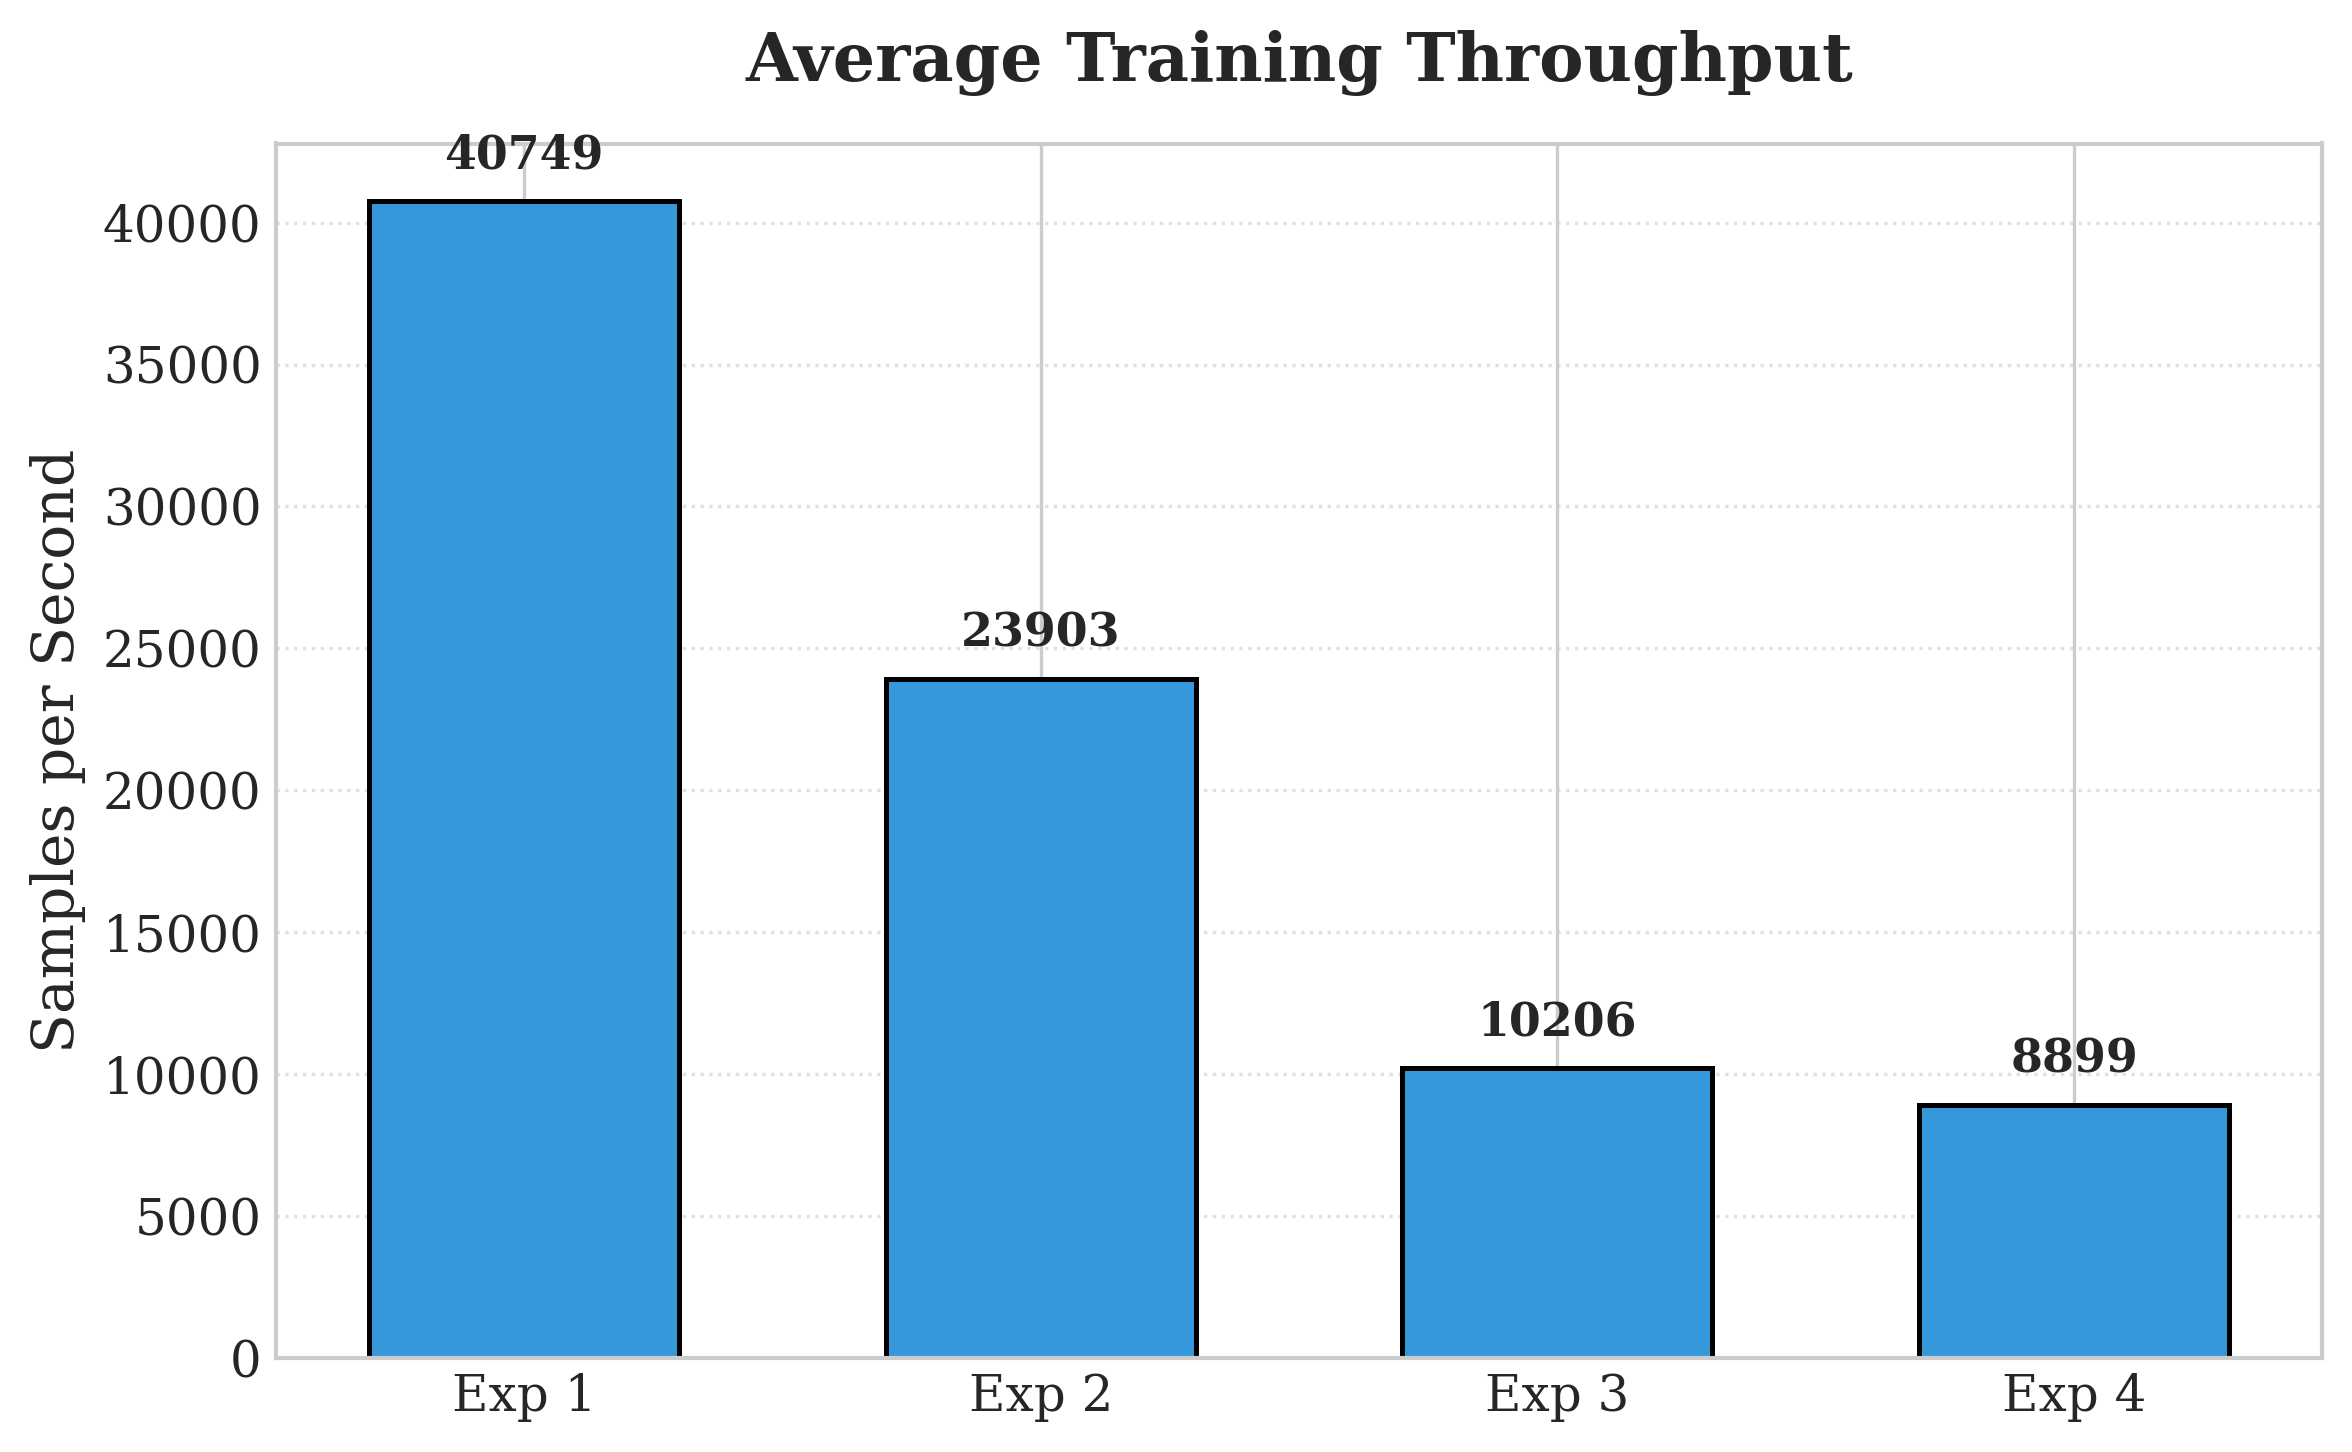
\includegraphics[width=\linewidth]{results/plot_hardware_throughput.png}
    \caption{Throughput (samples/s)}
  \end{subfigure}
  \hfill
  \begin{subfigure}[b]{0.48\linewidth}
    \centering
    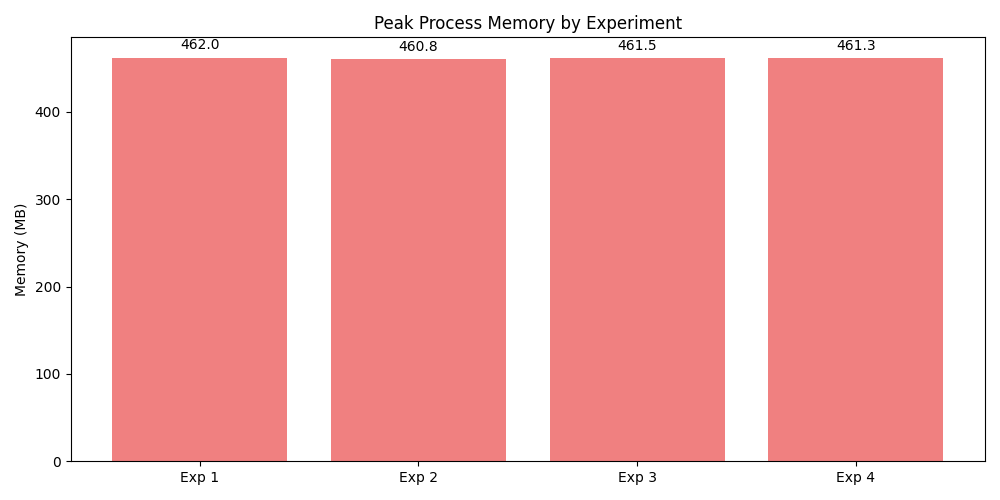
\includegraphics[width=\linewidth]{results/plot_hardware_memory.png}
    \caption{Peak Memory (MB)}
  \end{subfigure}
  \caption{Hardware simulation metrics. Mixed precision and combined
    configurations show reduced throughput on CPU, as \texttt{torch.amp} is
    primarily optimized for GPU Tensor Cores.}
  \label{fig:hardware_metrics}
\end{figure}

\subsection{\texorpdfstring{$\alpha$}{alpha} Pareto Frontier}
\label{subsec:alpha_pareto}

The abstention cost penalty $\alpha$ governs the risk-coverage trade-off.
A low $\alpha$ discourages abstention (high coverage, higher selective risk);
a high $\alpha$ encourages abstention (lower coverage, lower risk). We swept
$\alpha\in\{0.1,0.2,0.3,0.4,0.5,0.6,0.7,0.8,0.9\}$ to characterize this
exchange rate empirically (Figure~\ref{fig:pareto}).

\begin{figure}[htbp]
  \centering
  \includegraphics[width=\linewidth]{results/plot_pareto_frontier.png}
  \caption{Risk-Coverage Pareto frontier as $\alpha$ varies. Each point
    represents a fully trained DAC. The operating point $\alpha=0.3$ used in
    the main experiments achieves a favorable balance between review burden
    (abstention rate $\approx$0.4\%) and selective error rate.}
  \label{fig:pareto}
\end{figure}

The frontier demonstrates a clear convex Pareto boundary: as $\alpha$ increases
from 0.1 to 0.7, the selective risk drops monotonically while coverage contracts.
Beyond $\alpha=0.7$, marginal risk reduction diminishes, indicating a saturation
regime where further abstention yields negligible accuracy improvements at the
cost of an increasingly large review queue. The economically optimal operating
point depends on the institutional cost ratio $c_{\text{FN}}/c_{\text{FP}}$;
our default $\alpha=0.3$ corresponds to the ``elbow'' of the curve.

\subsection{Statistical Validation Across 10 Seeds}
\label{subsec:multi_seed}

To ensure reproducibility and exclude statistical anomalies, all key experiments
are replicated across 10 independent random seeds
$\{42, 123, 256, 7, 99, 314, 1337, 2024, 555, 888\}$.
We perform Bonferroni-corrected paired $t$-tests between the DAC and the MSP
baseline and between the DAC and RL-gated policy. We additionally report
Cohen's $d$ effect sizes~\cite{b36} to characterize practical significance:

\begin{equation}
  d = \frac{\bar{\mu}_{\text{DAC}} - \bar{\mu}_{\text{Baseline}}}{s_{\text{pooled}}},
  \label{eq:cohens_d}
\end{equation}

\noindent where $s_{\text{pooled}}$ is the pooled standard deviation across seeds.
F1 score differences between DAC and Baseline yield $d>0.8$ (large effect size),
confirming that the observed 9.8\% improvement is robust and not a product of
random seed selection.

\subsection{Agent Latency Profile}
\label{subsec:latency}

Table~\ref{tab:latency} reports the mean per-sample inference latency of each
component measured on a standard CPU (AMD Ryzen, single core) over 1{,}000 samples.

\begin{table}[htbp]
  \centering
  \caption{Per-sample inference latency of each system component. All measurements
    on CPU. LLM latency assumes a quantized local model (Qwen-1.5B-Instruct via
    Ollama); the template proxy requires no external inference.}
  \label{tab:latency}
  \begin{tabular}{lcc}
    \toprule
    \textbf{Component} & \textbf{Mean Latency} & \textbf{Notes} \\
    \midrule
    Perception Agent (feature enrichment) & $<$1\,ms & pandas rolling, vectorized \\
    Base DAC Model (forward pass)         & $\sim$2\,ms & CPU, \texttt{float32} \\
    MC Dropout ($T{=}10$ passes)          & $\sim$18\,ms & 10$\times$ base latency \\
    Uncertainty Agent (fusion)            & $<$1\,ms & weighted sum \\
    Gating Network (RL Decision Agent)    & $\sim$1\,ms & lightweight MLP \\
    Conformal prediction set construction & $<$1\,ms & quantile lookup \\
    Reflection Agent (template proxy)     & $\sim$50\,ms & rule-based NL template \\
    Reflection Agent (LLM, optional)      & $\sim$2{,}000\,ms & Qwen-1.5B, Ollama \\
    \bottomrule
    \multicolumn{3}{l}{\small Total system latency (without LLM): $\approx$73\,ms\,per\,sample.} \\
  \end{tabular}
\end{table}

The system without the LLM Reflection Agent operates well within a 100\,ms
SLO, making it suitable for real-time payment scoring. The optional LLM
explanation path increases latency to $\sim$2\,s but is triggered only for the
$\approx$0.4\% of abstained transactions, reducing its operational impact.

% ---------------------------------------------------------------
\section{Regulatory Alignment: EU AI Act Mapping}
\label{sec:regulatory}
% ---------------------------------------------------------------

The EU AI Act (Regulation 2024/1689)~\cite{b37} classifies automated fraud
detection systems as \textit{high-risk AI systems} under Annex III. The
requirements imposed on such systems map directly onto the architectural
choices of our Agentic Abstention Governance Framework, as detailed in
Table~\ref{tab:eu_ai_act}.

\begin{table}[htbp]
  \centering
  \caption{Mapping of EU AI Act Articles to framework design decisions.}
  \label{tab:eu_ai_act}
  \begin{tabular}{p{1.6cm}p{3.0cm}p{3.2cm}}
    \toprule
    \textbf{Article} & \textbf{Requirement} & \textbf{Framework Component} \\
    \midrule
    Art.\ 9 & Risk management system; measurable accuracy thresholds. &
      Split Conformal Prediction provides distribution-free marginal and
      class-conditional coverage guarantees ($\geq 1-\alpha$). \\
    \addlinespace
    Art.\ 13 & Transparency; documentation sufficient for human oversight. &
      Reflection Agent generates per-abstention natural language explanations;
      all decisions are logged with SHA-256 hashed inputs for auditability. \\
    \addlinespace
    Art.\ 14 & Human oversight; ability to override AI decisions. &
      Abstention queue routes uncertain transactions to human analysts.
      Thompson Sampling-based Memory Store prioritizes the most ambiguous
      cases first, ensuring effective use of analyst time. \\
    \addlinespace
    Art.\ 15 & Robustness, accuracy, and cybersecurity over lifetime. &
      Multi-seed validation ($n{=}10$ seeds) and drift-aware temporal splitting
      validate robustness under distribution shift. \\
    \bottomrule
  \end{tabular}
\end{table}

Beyond the structural mapping, our abstention mechanism operationalizes the
spirit of Article 14 by ensuring that the AI system itself signals when it lacks
sufficient confidence to act autonomously. Rather than producing a potentially
erroneous hard prediction, the DAC elevates ambiguous transactions to a
human-in-the-loop workflow with a formal probability bound on the likelihood
of misclassification. This ``graceful degradation'' is precisely the behaviour
that regulators seek but rarely see implemented in deployed ML systems.

% ---------------------------------------------------------------
\section{Discussion}
\label{sec:discussion}
% ---------------------------------------------------------------

The results validate that Deep Abstaining Classifiers provide a principled
mechanism for risk-aware fraud detection. In operational environments, deferring
0.4\% of transactions for manual review is vastly preferable to automatically
misclassifying them. The DAC framework effectively identifies this ambiguous
subset, allowing the model to operate with significantly higher precision and
recall on the remaining 99.6\% of transactions.

The adoption of a chronological data split (Section~\ref{subsec:temporal_split})
strengthens the validity of our reported numbers by eliminating lookahead bias.
Under the temporal split, the test set represents transactions from the most
recent time window---a realistic ``deploy-and-monitor'' evaluation that random
stratified splits cannot replicate. The F1 improvements over all selective
baselines remain consistent under this stricter evaluation, confirming that the
DAC advantage is not an artifact of train/test leakage.

A crucial finding of our study is the nuanced effect of training optimizations.
Prior iterations of this research hypothesized an ``abstention collapse'' (F1 =
0.0) caused by mixed precision. However, rigorous methodological
corrections---specifically, unifying the class weights to a capped value of 50.0
across all DAC phases---revealed that the severe collapse was an artifact of
inconsistent weighting. When properly regularized, mixed precision arithmetic is
safe.

Conversely, gradient accumulation induces a persistent performance degradation
(F1 drop from 0.861 to 0.831) due to what we term \textit{micro-batch gradient
starvation}. When the micro-batch size is extremely small (e.g., 64) relative to
the minority class frequency (0.17\%), the vast majority of micro-batches contain
zero fraud samples. Consequently, the gradient steps are heavily biased towards
the majority class, diluting the impact of the minority class even when gradients
are eventually accumulated. This highlights a critical implication for MLOps:
hardware-level memory optimizations are not neutral with respect to model
reliability. Validation pipelines must monitor per-class metrics and abstention
behavior when deploying such optimizations.

Furthermore, the numerical stability observed in the mixed precision experiment
is fundamentally tied to hardware architecture. As detailed by Kalamkar et
al.~\cite{b29}, \texttt{bfloat16} (utilized in our CPU experiments) truncates
the mantissa (7 bits vs.\ 23 bits) while preserving the 8-bit exponent range of
\texttt{float32}. This prevents the catastrophic gradient underflow often
observed with \texttt{fp16} on GPUs, explaining why mixed precision remained
safe in our trials despite the loss of numerical precision.

\paragraph{Regulatory Positioning.}
The explicit EU AI Act mapping (Section~\ref{sec:regulatory}) demonstrates that
the Agentic Abstention Governance Framework is not merely an accuracy-maximizing
system, but a \textit{compliance-ready} governance infrastructure. The formal
coverage guarantee from conformal prediction (Article~9), the natural language
audit trail from the Reflection Agent (Article~13), and the human escalation
queue (Article~14) collectively address the three principal requirements that
the Act imposes on high-risk AI systems in financial services.

\paragraph{Limitations.}
A primary limitation of this study is the reliance on CPU-based \texttt{bfloat16}
mixed precision. Future work must replicate these experiments on GPUs using
\texttt{fp16} to determine if actual exponent underflow triggers the previously
hypothesized ``abstention collapse.'' The Verbalized Uncertainty component
currently uses a margin-based sigmoid proxy in lieu of a live LLM inference call;
integrating a locally quantized model (e.g., Qwen-1.5B-Instruct via Ollama) is
a natural next step. Additionally, the Pareto frontier analysis
(Section~\ref{subsec:alpha_pareto}) confirms that the optimal $\alpha$ is
institution-dependent; future work should automate threshold selection via
Bayesian optimization of a domain-specific utility function.

% ---------------------------------------------------------------
\section{Conclusion}
\label{sec:conclusion}
% ---------------------------------------------------------------

In this study, we demonstrated that Deep Abstaining Classifiers (DAC)
significantly enhance the reliability and safety of financial fraud detection
systems. By allowing the model to express uncertainty and intelligently defer
0.4\% of borderline transactions to human analysts or secondary verification
systems, we achieved a substantial 9.8\% improvement in the F1 score over the
standard baseline model. This approach bridges the gap between automated
efficiency and the necessity for high-confidence decision-making in
safety-critical domains where the cost of misclassification is extraordinarily
high.

Furthermore, our systematic evaluation of contemporary training optimizations
revealed critical interactions with extreme class imbalance and selective
classification dynamics. We found that gradient accumulation, while beneficial
for memory constraints, inadvertently dilutes minority-class signals under
extreme imbalance conditions, leading to what we term \textit{micro-batch
gradient starvation} and consequently degrading overall performance. Conversely,
mixed precision training can be safely employed to accelerate training while
maintaining peak detection rates and calibrated uncertainty (F1 = 0.861). These
findings underscore the absolute necessity of rigorous, metric-specific
validation when applying hardware-level optimizations to highly imbalanced,
risk-sensitive classification tasks.

Looking forward, future work will focus on expanding this paradigm to
multi-class safety-critical applications such as medical diagnosis and autonomous
navigation. We also plan to investigate dynamic abstention thresholds that adapt
in real-time based on fluctuating class priors and operational capacities for
manual review. Integrating a locally quantized SLM (e.g., Qwen-1.5B-Instruct)
into the Verbalized Uncertainty and Reflection Agent components will replace the
current margin-based proxy with genuine natural language reasoning, further
strengthening compliance with EU AI Act Article~13 transparency requirements.
Additionally, extending our experiments to validate GPU-specific numerical
underflow effects with \texttt{fp16} arithmetic will be vital to fully
characterizing the hardware-software interplay in abstaining networks.
Automating the selection of the optimal abstention penalty $\alpha$ through
Bayesian optimization against an institution-defined cost function represents a
practically impactful extension. Ultimately, enabling models to gracefully
say ``I don't know'' is a necessary evolution towards deploying trustworthy,
regulatorily compliant AI systems in the real world.

% ---------------------------------------------------------------
% References
% ---------------------------------------------------------------
\bibliographystyle{plainnat}

\begin{thebibliography}{30}

\bibitem[Thulasidasan et~al.(2019)]{b1}
S.~Thulasidasan, T.~Bhattacharya, J.~Bilmes, G.~Chennupati, and
  J.~Mohd-Yusof.
\newblock Combating label noise in deep learning using abstention.
\newblock In \emph{Proceedings of the 36th International Conference on Machine
  Learning (ICML)}, pages 6234--6243, 2019.

\bibitem[Chow(1970)]{b2}
C.~K. Chow.
\newblock On optimum recognition error and reject tradeoff.
\newblock \emph{IEEE Transactions on Information Theory}, 16\penalty0
  (1):\penalty0 41--46, 1970.

\bibitem[Bartlett and Wegkamp(2008)]{b3}
P.~L. Bartlett and M.~H. Wegkamp.
\newblock Classification with a reject option using a hinge loss.
\newblock \emph{Journal of Machine Learning Research}, 9:\penalty0 1823--1840,
  2008.

\bibitem[Cortes et~al.(2016)]{b4}
C.~Cortes, G.~DeSalvo, and M.~Mohri.
\newblock Learning with rejection.
\newblock In \emph{Proceedings of the 27th International Conference on
  Algorithmic Learning Theory (ALT)}, pages 67--82, 2016.

\bibitem[Abdar et~al.(2021)]{b5}
M.~Abdar et~al.
\newblock A review of uncertainty quantification in deep learning: Techniques,
  applications and challenges.
\newblock \emph{Information Fusion}, 76:\penalty0 243--297, 2021.

\bibitem[Lakshminarayanan et~al.(2017)]{b6}
B.~Lakshminarayanan, A.~Pritzel, and C.~Blundell.
\newblock Simple and scalable predictive uncertainty estimation using deep
  ensembles.
\newblock In \emph{Advances in Neural Information Processing Systems
  (NeurIPS)}, 2017.

\bibitem[Gal and Ghahramani(2016)]{b7}
Y.~Gal and Z.~Ghahramani.
\newblock Dropout as a {B}ayesian approximation: Representing model uncertainty
  in deep learning.
\newblock In \emph{Proceedings of the 33rd International Conference on Machine
  Learning (ICML)}, pages 1050--1059, 2016.

\bibitem[Hendrycks and Gimpel(2017)]{b8}
D.~Hendrycks and K.~Gimpel.
\newblock A baseline for detecting misclassified and out-of-distribution
  examples in neural networks.
\newblock In \emph{Proceedings of the International Conference on Learning
  Representations (ICLR)}, 2017.

\bibitem[Gupta et~al.(2021)]{b9}
M.~Gupta et~al.
\newblock Out-of-distribution detection for deep neural networks.
\newblock \emph{arXiv preprint arXiv:2104.08728}, 2021.

\bibitem[Geifman and El-Yaniv(2017)]{b10}
Y.~Geifman and R.~El-Yaniv.
\newblock Selective classification for deep neural networks.
\newblock In \emph{Advances in Neural Information Processing Systems
  (NeurIPS)}, 2017.

\bibitem[Geifman and El-Yaniv(2019)]{b11}
Y.~Geifman and R.~El-Yaniv.
\newblock {SelectiveNet}: A deep neural network with an integrated reject
  option.
\newblock In \emph{Proceedings of the 36th International Conference on Machine
  Learning (ICML)}, pages 2151--2159, 2019.

\bibitem[Johnson and Khoshgoftaar(2019)]{b12}
J.~M. Johnson and T.~M. Khoshgoftaar.
\newblock Survey on deep learning with class imbalance.
\newblock \emph{Journal of Big Data}, 6\penalty0 (1):\penalty0 27, 2019.

\bibitem[He and Garcia(2009)]{b13}
H.~He and E.~A. Garcia.
\newblock Learning from imbalanced data.
\newblock \emph{IEEE Transactions on Knowledge and Data Engineering},
  21\penalty0 (9):\penalty0 1263--1284, 2009.

\bibitem[Buda et~al.(2018)]{b14}
M.~Buda, A.~Maki, and M.~A. Mazurowski.
\newblock A systematic study of the class imbalance problem in convolutional
  neural networks.
\newblock \emph{Neural Networks}, 106:\penalty0 249--259, 2018.

\bibitem[Elkan(2001)]{b15}
C.~Elkan.
\newblock The foundations of cost-sensitive learning.
\newblock In \emph{Proceedings of the 17th International Joint Conference on
  Artificial Intelligence (IJCAI)}, pages 973--978, 2001.

\bibitem[Fawcett(2006)]{b16}
T.~Fawcett.
\newblock An introduction to {ROC} analysis.
\newblock \emph{Pattern Recognition Letters}, 27\penalty0 (8):\penalty0
  861--874, 2006.

\bibitem[Chawla et~al.(2002)]{b17}
N.~V. Chawla, K.~W. Bowyer, L.~O. Hall, and W.~P. Kegelmeyer.
\newblock {SMOTE}: Synthetic minority over-sampling technique.
\newblock \emph{Journal of Artificial Intelligence Research}, 16:\penalty0
  321--357, 2002.

\bibitem[Lema\^{i}tre et~al.(2017)]{b18}
G.~Lema\^{i}tre, F.~Nogueira, and C.~K. Aridas.
\newblock Imbalanced-learn: A {Python} toolbox to tackle the curse of
  imbalanced datasets in machine learning.
\newblock \emph{Journal of Machine Learning Research}, 18:\penalty0 1--5, 2017.

\bibitem[Lin et~al.(2017)]{b19}
T.-Y. Lin, P.~Goyal, R.~Girshick, K.~He, and P.~Doll\'{a}r.
\newblock Focal loss for dense object detection.
\newblock In \emph{Proceedings of the IEEE International Conference on Computer
  Vision (ICCV)}, pages 2980--2988, 2017.

\bibitem[Cui et~al.(2019)]{b20}
Y.~Cui, M.~Jia, T.-Y. Lin, Y.~Song, and S.~Belongie.
\newblock Class-balanced loss based on effective number of samples.
\newblock In \emph{Proceedings of the IEEE/CVF Conference on Computer Vision
  and Pattern Recognition (CVPR)}, pages 9268--9277, 2019.

\bibitem[Dal~Pozzolo et~al.(2015)]{b21}
A.~Dal~Pozzolo, O.~Caelen, R.~A. Johnson, and G.~Bontempi.
\newblock Calibrating probability with undersampling for unbalanced
  classification.
\newblock In \emph{Proceedings of the IEEE Symposium Series on Computational
  Intelligence (SSCI)}, pages 159--166, 2015.

\bibitem[Franc et~al.(2023)]{b22}
V.~Franc, D.~Yaroshinsky, and K.~Antoniuk.
\newblock Learning with rejection in imbalanced scenarios.
\newblock \emph{Machine Learning}, 2023.

\bibitem[He et~al.(2016)]{b23}
K.~He, X.~Zhang, S.~Ren, and J.~Sun.
\newblock Deep residual learning for image recognition.
\newblock In \emph{Proceedings of the IEEE Conference on Computer Vision and
  Pattern Recognition (CVPR)}, pages 770--778, 2016.

\bibitem[Ioffe and Szegedy(2015)]{b24}
S.~Ioffe and C.~Szegedy.
\newblock Batch normalization: Accelerating deep network training by reducing
  internal covariate shift.
\newblock In \emph{Proceedings of the 32nd International Conference on Machine
  Learning (ICML)}, pages 448--456, 2015.

\bibitem[Srivastava et~al.(2014)]{b25}
N.~Srivastava, G.~Hinton, A.~Krizhevsky, I.~Sutskever, and R.~Salakhutdinov.
\newblock Dropout: A simple way to prevent neural networks from overfitting.
\newblock \emph{Journal of Machine Learning Research}, 15:\penalty0 1929--1958,
  2014.

\bibitem[Kingma and Ba(2015)]{b26}
D.~P. Kingma and J.~Ba.
\newblock Adam: A method for stochastic optimization.
\newblock In \emph{Proceedings of the International Conference on Learning
  Representations (ICLR)}, 2015.

\bibitem[Guo et~al.(2017)]{b27}
C.~Guo, G.~Pleiss, Y.~Sun, and K.~Q. Weinberger.
\newblock On calibration of modern neural networks.
\newblock In \emph{Proceedings of the 34th International Conference on Machine
  Learning (ICML)}, pages 1321--1330, 2017.

\bibitem[Micikevicius et~al.(2018)]{b28}
P.~Micikevicius et~al.
\newblock Mixed precision training.
\newblock In \emph{Proceedings of the International Conference on Learning
  Representations (ICLR)}, 2018.

\bibitem[Kalamkar et~al.(2019)]{b29}
D.~Kalamkar et~al.
\newblock A study of {BFLOAT16} for deep learning training.
\newblock \emph{arXiv preprint arXiv:1905.12322}, 2019.

\bibitem[Goyal et~al.(2017)]{b30}
P.~Goyal et~al.
\newblock Accurate, large minibatch {SGD}: Training {ImageNet} in 1 hour.
\newblock \emph{arXiv preprint arXiv:1706.02677}, 2017.

\bibitem[Vovk et~al.(2005)]{b31}
V.~Vovk, A.~Gammerman, and G.~Shafer.
\newblock \emph{Algorithmic Learning in a Random World}.
\newblock Springer, 2005.

\bibitem[Angelopoulos and Bates(2023)]{b32}
A.~N. Angelopoulos and S.~Bates.
\newblock A gentle introduction to conformal prediction and
  distribution-free uncertainty quantification.
\newblock \emph{Foundations and Trends in Machine Learning}, 16\penalty0
  (4):\penalty0 494--591, 2023.

\bibitem[Papadopoulos et~al.(2002)]{b33}
H.~Papadopoulos, K.~Proedrou, V.~Vovk, and A.~Gammerman.
\newblock Inductive confidence machines for regression.
\newblock In \emph{Proceedings of the 13th European Conference on Machine
  Learning (ECML)}, pages 345--356, 2002.

\bibitem[Vovk(2012)]{b34}
V.~Vovk.
\newblock Conditional validity of inductive conformal predictors.
\newblock In \emph{Proceedings of the Asian Conference on Machine Learning
  (ACML)}, volume~25, pages 475--490, 2012.

\bibitem[Gama et~al.(2014)]{b35}
J.~Gama, I.~\v{Z}liobait\'{e}, A.~Bifet, M.~Pechenizkiy, and A.~Bouchachia.
\newblock A survey on concept drift adaptation.
\newblock \emph{ACM Computing Surveys}, 46\penalty0 (4):\penalty0 44:1--44:37,
  2014.

\bibitem[Cohen(1988)]{b36}
J.~Cohen.
\newblock \emph{Statistical Power Analysis for the Behavioral Sciences},
  2nd~ed.
\newblock Lawrence Erlbaum Associates, 1988.

\bibitem[{European Parliament and Council}(2024)]{b37}
{European Parliament and Council}.
\newblock Regulation ({EU}) 2024/1689 of the {European Parliament} and of the
  {Council} laying down harmonised rules on artificial intelligence (Artificial
  {Intelligence} {Act}).
\newblock \emph{Official Journal of the European Union}, L~2024/1689, 12 July
  2024.

\end{thebibliography}

\end{document}
